\documentclass[11pt]{article}

\usepackage[margin=1in]{geometry}
\usepackage{graphicx}
\usepackage{amsmath}
\usepackage{booktabs}
\usepackage[round,authoryear]{natbib}
\usepackage{hyperref}

\graphicspath{{figures/}{../figures/}}

\hypersetup{
  colorlinks=true,
  linkcolor=blue!50!black,
  citecolor=blue!50!black,
  urlcolor=blue!50!black
}

\newcommand{\teff}{t_{\mathrm{eff}}}
\newcommand{\fwhm}{\mathrm{FWHM}}
\newcommand{\arcsecunit}{^{\prime\prime}}

\title{Evaluation Metrics and Rewards for AI-Based Telescope Schedulers\\
  \large A validated effective-exposure-time metric and per-night schedule scores on real DES data (v0.1)}
\author{Shain Carrasco\\ \small SkAI Institute}
\date{July 6, 2026}

\begin{document}

\maketitle

\begin{abstract}
Before we can train or even fairly compare AI schedulers for ground-based telescopes,
we need a number that says how good an observation---and a night of
observations---actually was. This note documents the first phase of that work. We
adopt the \emph{effective exposure time} $\teff$ of \citet{neilsen2019}, the same
quantity used as the reinforcement-learning reward by \citet{terranova2023}, and
reconstruct it from first principles directly from the quality columns of the public
DES exposure log (105{,}889 exposures, 2013--2019). A per-band calibration of the
fiducial seeing and of an empirical sky-brightness term brings our reconstruction to
a log-correlation of $0.95$ against the DES pipeline's own $\teff$, with a median
relative error of $15\%$ (versus $24\%$ for uncalibrated paper constants); the
fitted fiducials independently recover the atmospheric $\lambda^{-0.2}$ law. Decomposing
the blur term, we find a striking selection effect: pooled over all exposures, image
blur apparently \emph{improves} with airmass (fitted exponent $-0.23$ instead of the
physical $+0.6$), because the DES scheduler preferentially pointed far from zenith on
nights of good seeing. Within-night fits recover the physical trend. This is
Simpson's paradox in scheduler logs, and it is direct evidence that evaluating
scheduling policies on logged data is confounded by the logging policy---precisely the
off-policy problem that motivates conservative offline RL. Finally, we aggregate
$\teff$ into per-night schedule metrics and a transparent composite score, and apply
them to 615 real DES nights. All code is packaged as the \texttt{skai\_metrics}
toolkit with four automated validation tests, all passing.
\end{abstract}

\section{Introduction and motivation}
\label{sec:intro}

Scheduling a ground-based telescope is a sequential decision problem of unpleasant
size. At every moment the scheduler must choose a pointing, a filter, and an exposure
time from a combinatorially large set of options, under observing conditions (seeing,
clouds, sky brightness) that evolve stochastically on timescales of minutes, and under
scientific constraints (cadence requirements, footprint coverage, airmass limits) that
couple decisions made hours or nights apart. The underlying optimization is NP-hard,
and production schedulers are, in practice, carefully hand-tuned heuristics.

Our group's research direction is to learn scheduling policies from data. Because a
telescope cannot be handed over to an untrained agent for millions of exploratory
episodes, the natural setting is \emph{offline} reinforcement learning: train on the
logs of an existing scheduler, without further interaction with the environment.
\citet{terranova2023} demonstrated the feasibility of this program by training a deep
$Q$-network to schedule the Stone Edge Observatory, using the effective exposure time
$\teff$ as the reward signal; on the algorithmic side, Conservative $Q$-Learning
\citep[CQL;][]{kumar2020} is the offline-RL method we intend to build on, since it is
designed to behave sensibly exactly where the logged data is silent.

Everything in this program---the reward the agent maximizes, the evaluation that
decides whether the learned policy beats the baseline, the diagnostics that tell us
\emph{why}---rests on one foundation: a quantitative, physically meaningful,
validated metric for how good an observation is. If the metric is wrong, the agent
will faithfully optimize the wrong thing. This document describes our first
contribution: the choice, physical derivation, empirical calibration, and validation
of that metric on real Dark Energy Survey (DES) data, and its aggregation into
schedule-level scores. We deliberately work through the physics from first principles;
part of the goal of this phase was for us to \emph{understand} the reward we are about
to hand to a learning agent, not merely to import it.

\section{Data: the DES exposure log}
\label{sec:data}

We work with \texttt{des-exposures.csv}, a public log of $105{,}889$ exposures taken
by the Dark Energy Camera (DECam) at the Blanco 4-m telescope, CTIO, between
2013-08-31 and 2019-01-10---essentially the full six-year Dark Energy Survey. Each row
is one exposure, with the columns most relevant to us:

\begin{itemize}
  \item \texttt{qc\_fwhm} --- delivered image full width at half maximum (arcsec), as
    measured by the DES quality pipeline: the ``blur'' of the exposure.
  \item \texttt{qc\_cloud} --- atmospheric extinction attributable to clouds. As we
    show in Section~\ref{sec:calibration}, this column is an extinction in
    \emph{magnitudes} (0 = photometric).
  \item \texttt{qc\_sky} --- sky-brightness excess over nominal dark sky. Empirically
    this behaves as a \emph{fractional} excess (0 = nominal dark sky; a bright moon
    can push it to tens).
  \item \texttt{teff} (and \texttt{qc\_teff}) --- the DES pipeline's own effective
    exposure time, our ground truth for validation.
  \item \texttt{airmass} --- the secant of the zenith angle at which the exposure was
    taken: the path length through the atmosphere relative to pointing straight up.
  \item \texttt{filter} --- the DECam band ($g,r,i,z,Y$, from blue to near-infrared).
  \item \texttt{program} --- which observing program the exposure served
    (\texttt{survey}, supernova fields, GW follow-up, engineering).
\end{itemize}

For calibration and per-night scoring we restrict to the homogeneous core of the
survey: \texttt{program == 'survey'} exposures with the standard 90\,s exposure time,
with quality cuts dropping rows carrying unphysical pipeline values (missing or
non-positive $\teff$; $\fwhm \le 0.4\arcsecunit$ or $\fwhm \ge 4\arcsecunit$; sky
excess $\le -0.9$; corrupt or epoch-zero timestamps). These cuts remove
sensor and pipeline artifacts, not real observations. The clean sample contains
$74{,}323$ exposures ($g$: 20{,}128; $r$: 18{,}032; $i$: 16{,}971; $z$: 15{,}629; $Y$:
3{,}563) spread over $615$ scoreable nights. Exposures are grouped into local
observing nights by shifting the UTC timestamps back 12 hours, so that a single dark
period is never split at midnight.

\section{The effective exposure time}
\label{sec:teff}

\subsection{The formula and where it comes from}

The metric we adopt is the effective exposure time of \citet{neilsen2019}:
\begin{equation}
  \teff \;=\; \eta^2 \,
  \left( \frac{\fwhm_{\mathrm{fid}}}{\fwhm} \right)^{2}
  \left( \frac{b_{\mathrm{dark}}}{b} \right),
  \label{eq:teff}
\end{equation}
where $\eta$ is the atmospheric transmission (unity in photometric conditions),
$\fwhm$ is the delivered image blur, $b$ is the sky background surface brightness,
and the ``fid''/``dark'' subscripts denote fiducial benchmark conditions.
Each factor, and in particular each \emph{exponent}, follows from the standard
signal-to-noise argument for a faint point source on a bright sky. It is worth
walking through, because the exponents are exactly what make $\teff$ a good reward.

Consider a point source of flux $F$ observed for clock time $\tau$. The detected
signal is $S \propto \eta F \tau$: photons are collected linearly in time, and clouds
remove a fraction $(1-\eta)$ of them. The source's light lands on the detector in a
seeing disk of diameter $\sim \fwhm$, i.e.\ spread over an area of
$n_{\mathrm{pix}} \propto \fwhm^2$ pixels. In the background-limited regime (the
regime of every faint-object survey), the noise is dominated by Poisson fluctuations
of the sky counts accumulated under the source footprint:
$N \propto \sqrt{b \, n_{\mathrm{pix}} \, \tau} \propto \fwhm \sqrt{b\,\tau}$.
Therefore
\begin{equation}
  \mathrm{SNR} \;=\; \frac{S}{N}
  \;\propto\; \frac{\eta F \tau}{\fwhm \sqrt{b\,\tau}}
  \qquad\Longrightarrow\qquad
  \mathrm{SNR}^2 \;\propto\; \frac{\eta^2}{\fwhm^{2}\, b}\;\tau .
  \label{eq:snr}
\end{equation}
Squared SNR---the statistically meaningful ``information content'' of the
exposure---accrues \emph{linearly in time}, with a proportionality constant set
entirely by conditions. Now ask: how long an exposure $\tau_{\mathrm{eff}}$ in
fiducial conditions ($\eta=1$, $\fwhm_{\mathrm{fid}}$, $b_{\mathrm{dark}}$) would
reach the same $\mathrm{SNR}^2$ as our actual exposure of length $\tau$? Setting the
two expressions equal and solving gives $\tau_{\mathrm{eff}} = \teff \cdot \tau$ with
$\teff$ exactly as in Eq.~\eqref{eq:teff}. The exponents are now transparent:

\begin{itemize}
  \item \textbf{Transmission enters squared} ($\eta^2$): the signal scales with
    $\eta$, and $\mathrm{SNR}^2$ scales with signal squared over noise---the sky
    noise does not care about the clouds dimming the source. Half a magnitude of
    cloud ($\eta = 10^{-0.4 \times 0.5}$) already costs 60\% of the exposure's value.
  \item \textbf{Blur enters squared}: a point source's flux is spread over an area
    $\propto \fwhm^2$, so the sky noise under the source grows linearly with
    $\fwhm$, and $\mathrm{SNR}^2$ falls as $\fwhm^{-2}$. Doubling the seeing
    quarters the worth of the exposure.
  \item \textbf{Sky brightness enters linearly}: it appears only in the noise
    variance, which is proportional to the background count rate.
\end{itemize}

\subsection{Why this is the natural scheduler reward}

The derivation gives $\teff$ a precise operational meaning: \emph{an exposure of
length $\tau$ taken in the given conditions detects point sources exactly as well as
an exposure of length $\teff\,\tau$ taken in fiducial conditions}. $\teff$ is a
multiplier on time itself. That interpretation is what elevates it from a quality
statistic to a reward: the quantity
\begin{equation}
  \sum_{\mathrm{exposures}} \teff \cdot \tau
  \label{eq:effective-seconds}
\end{equation}
is the night's \emph{effective open-shutter time}---science-grade seconds in a common
currency---and a scheduler that maximizes it is maximizing precisely the resource a
survey exists to collect. Rewards in different bands, sky conditions, and moon phases
all become commensurable seconds. This is the quantity \citet{terranova2023} used as
the per-step DQN reward, and the quantity we adopt.

DES itself uses $\teff$ operationally: exposures falling below per-band thresholds
($\teff < 0.2$ in $g$ and $Y$; $\teff < 0.3$ in $r,i,z$) do not count toward survey
completion and are retaken \citep{neilsen2019}. These thresholds give us a natural
per-exposure pass/fail criterion that we reuse in Section~\ref{sec:schedule}.

\section{Empirical calibration and validation}
\label{sec:calibration}

Eq.~\eqref{eq:teff} is a physical form, not yet a computable function of the CSV
columns: we must identify what \texttt{qc\_cloud} and \texttt{qc\_sky} actually
measure and what fiducial values DES used. Rather than trusting constants quoted in
papers, we fit everything on the data and let the DES pipeline's own
\texttt{qc\_teff} arbitrate. This section is the heart of the phase-one work. All
comparisons below use log-space correlation, since $\teff$ spans more than two
decades and multiplicative errors are the relevant ones.

\subsection{Step 1: the blur $\times$ cloud core identifies \texttt{qc\_cloud}}

We first test the hypothesis that \texttt{qc\_cloud} is a cloud extinction in
magnitudes, so that $\eta^2 = 10^{-0.8\,c}$. Using only the blur and cloud factors,
\begin{equation}
  \teff^{\mathrm{core}} = 10^{-0.8\,c}\left(\frac{\fwhm_{\mathrm{fid}}}{\fwhm}\right)^{2},
\end{equation}
already reproduces the pipeline $\teff$ with a log-correlation of $0.93$ across the
full clean sample. This simultaneously confirms the magnitude interpretation of
\texttt{qc\_cloud} and shows the multiplicative structure of Eq.~\eqref{eq:teff} is
the right skeleton; the residual scatter must be carried by the sky term.

\subsection{Step 2: per-band fiducial seeing---and a consistency check against physics}

The fiducial $\fwhm_{\mathrm{fid}}$ is band-dependent (bluer light is blurred more by
the atmosphere), and its values are a convention baked into the DES pipeline. We fit
them per band by requiring our reconstruction to match \texttt{qc\_teff} in the
median. The results are listed in Table~\ref{tab:calibration}.

\begin{table}[htbp]
  \centering
  \caption{Per-band calibration fit on the clean 90\,s survey sample. Fiducial FWHM
    is the seeing at which the blur term equals unity; $\alpha_b$ is the exponent of
    the empirical sky term $(1+\Delta b)^{-\alpha_b}$; the last row gives the DES
    keep-or-retake threshold on $\teff$ \citep{neilsen2019}.}
  \label{tab:calibration}
  \begin{tabular}{lccccc}
    \toprule
     & $g$ & $r$ & $i$ & $z$ & $Y$ \\
    \midrule
    Fiducial FWHM (arcsec)      & 1.119 & 0.991 & 0.932 & 0.871 & 0.904 \\
    Sky exponent $\alpha_b$     & 0.589 & 0.487 & 0.254 & 0.213 & 0.881 \\
    $\teff$ threshold           & 0.2   & 0.3   & 0.3   & 0.3   & 0.2   \\
    \bottomrule
  \end{tabular}
\end{table}

These fitted numbers carry an independent physics check. Kolmogorov turbulence theory
predicts that seeing scales with wavelength as $\fwhm \propto \lambda^{-1/5}$;
if our fitted fiducials are physically meaningful they should trace this law across
the five DECam bands ($\lambda_{\mathrm{eff}} = 475$, $635$, $775$, $925$, $1000$\,nm
for $g,r,i,z,Y$). They do (Figure~\ref{fig:fiducial-lambda}): four of the five bands
fall on the $\lambda^{-0.2}$ line, with $Y$ the mild outlier---plausibly because $Y$
is used mostly in bright time and contributes the smallest sample. Fitting constants
on data and \emph{rediscovering} an atmospheric scaling law we did not impose is the
kind of consistency that makes us trust the calibration.

\begin{figure}[htbp]
  \centering
  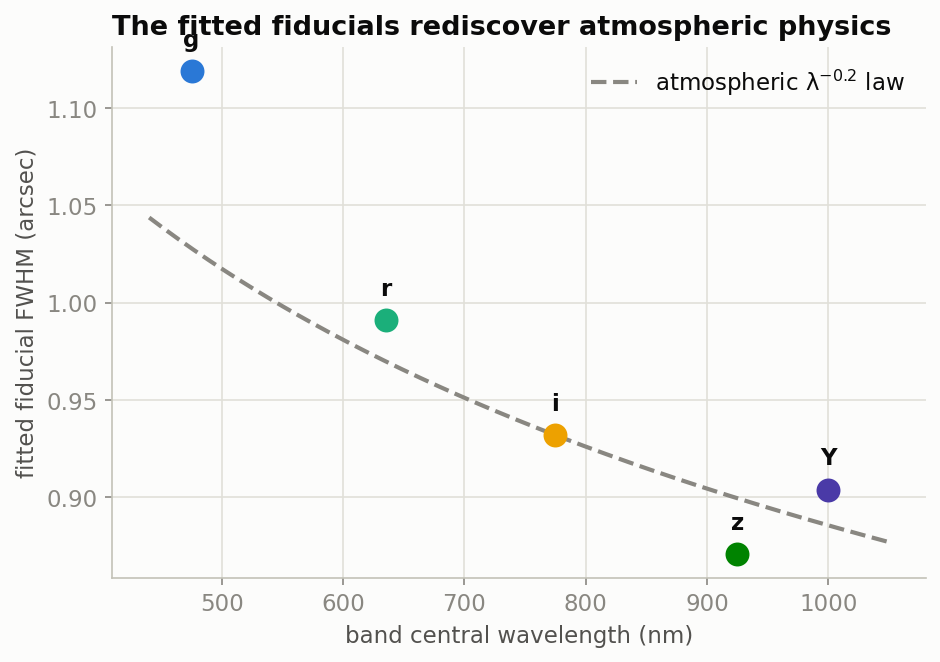
\includegraphics[width=0.72\textwidth]{fiducial_lambda.png}
  \caption{Fiducials rediscover physics: the per-band fiducial FWHM, fit purely to
    match the DES pipeline $\teff$, follows the atmospheric $\lambda^{-0.2}$ law.}
  \label{fig:fiducial-lambda}
\end{figure}

\subsection{Step 3: an empirical sky term}

The released \texttt{qc\_sky} column is not a surface brightness in physical units;
it behaves as a \emph{fractional} excess $\Delta b$ over nominal dark sky. The ideal
sky factor $b_{\mathrm{dark}}/b$ would then be $(1+\Delta b)^{-1}$, but the pipeline's
$\teff$ is evidently computed from a sky model that responds differently per band
(the sky spectrum, the detector response, and the definition of ``nominal'' all vary
with filter). We therefore adopt the empirical form
\begin{equation}
  \text{sky term} = (1+\Delta b)^{-\alpha_b},
\end{equation}
with one exponent per band, fit against \texttt{qc\_teff} with the blur and cloud
terms in place. The fitted $\alpha_b$ (Table~\ref{tab:calibration}) are largest in
$g$ and $Y$ and smallest in $z$---consistent with moonlight contaminating the blue
bands most strongly while $z$ is dominated by airglow, though we treat $\alpha_b$ as
calibration constants rather than over-interpreting them.

\subsection{Step 4: validation against the DES pipeline}

Figure~\ref{fig:teff-validation} shows the full calibrated reconstruction against the
pipeline's \texttt{qc\_teff} across all $74{,}323$ clean exposures, and
Figure~\ref{fig:teff-terms} shows the three factors individually as multipliers on
exposure time. The headline validation numbers:

\begin{table}[htbp]
  \centering
  \caption{Validation of the reconstructed $\teff$ against the DES pipeline value,
    over 74{,}323 clean 90\,s survey exposures.}
  \label{tab:validation}
  \begin{tabular}{lcc}
    \toprule
    Model & log-correlation & median $|$relative error$|$ \\
    \midrule
    Blur $\times$ cloud core only         & 0.933 & --- \\
    Naive paper constants (no calibration) & ---   & 23.9\% \\
    \textbf{Full calibrated model}         & \textbf{0.952} & \textbf{14.8\%} \\
    \bottomrule
  \end{tabular}
\end{table}

The calibration buys a substantial improvement over plugging in nominal constants:
the median relative error drops from $23.9\%$ to $14.8\%$, and the log-correlation
reaches $0.952$. The remaining scatter is consistent with the pieces we cannot see
from the released columns (the pipeline's full sky model and any per-CCD effects) and
is small compared to the dynamic range of $\teff$ itself, which spans from clouded-out
($\teff \approx 0.02$) to better-than-fiducial ($\teff > 1.5$) conditions.

The entire calibration is packaged in the \texttt{skai\_metrics} toolkit
(\texttt{teff.py}, \texttt{blur.py}, \texttt{schedule.py}, \texttt{data.py}) together
with an automated test suite that re-derives these checks from the raw CSV; all
\textbf{4 of 4 validation tests pass}, so the numbers in this section are
reproducible with one command.

\begin{figure}[htbp]
  \centering
  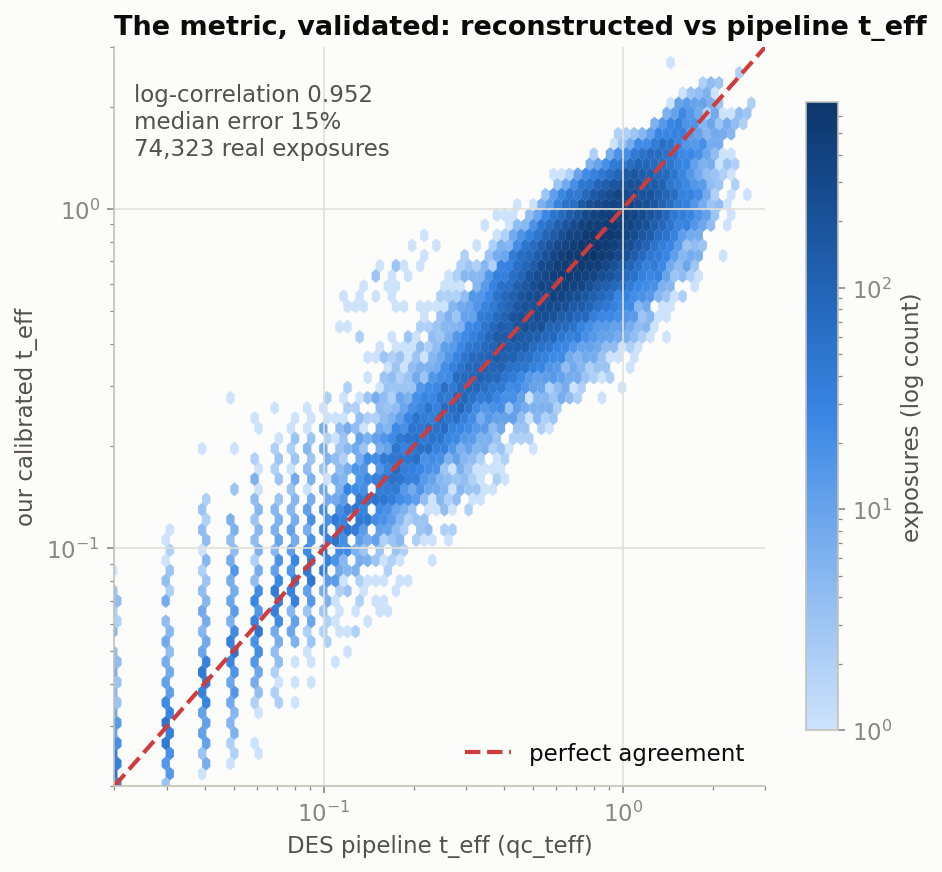
\includegraphics[width=0.8\textwidth]{teff_validation.png}
  \caption{Reconstructed vs.\ pipeline $\teff$: our calibrated metric against DES's
    own quality pipeline across 74{,}323 exposures---log-correlation 0.952.}
  \label{fig:teff-validation}
\end{figure}

\begin{figure}[htbp]
  \centering
  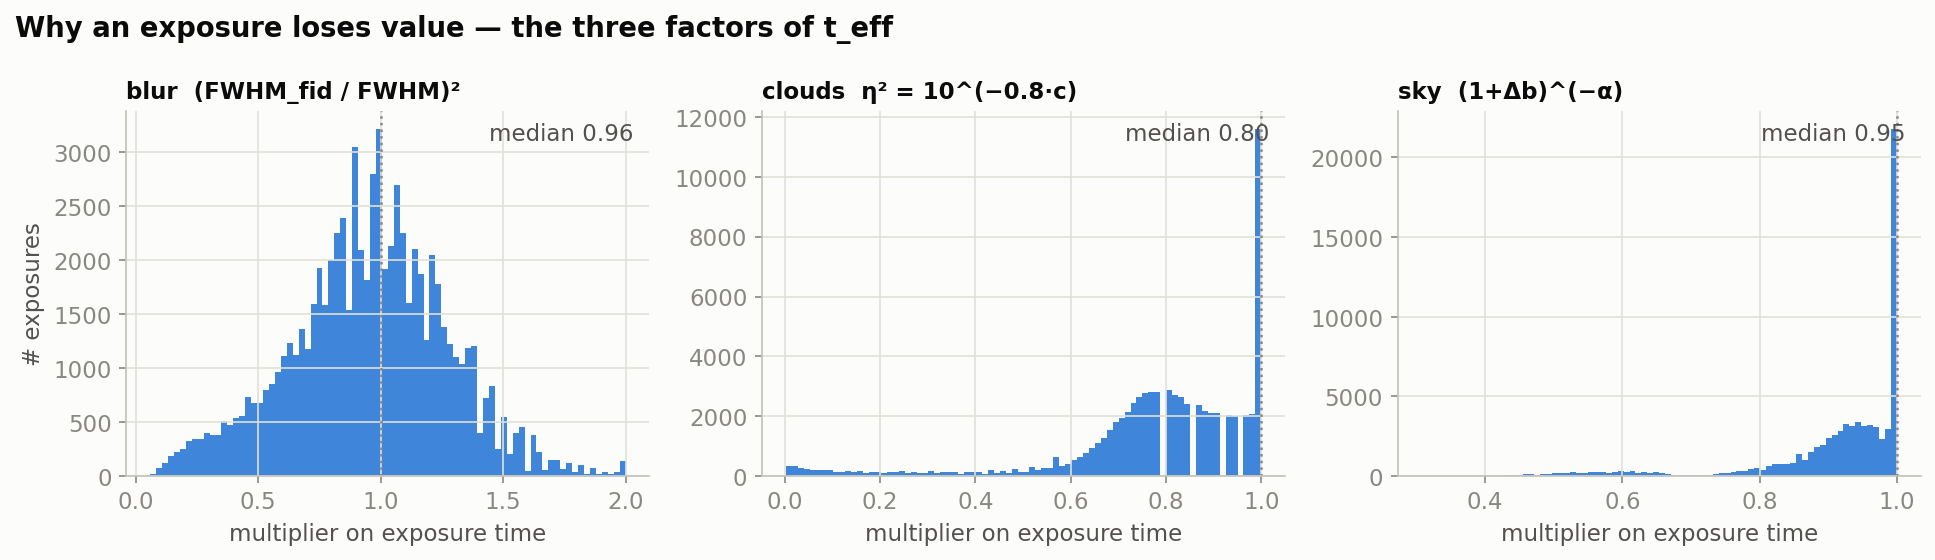
\includegraphics[width=0.95\textwidth]{teff_terms.png}
  \caption{The three factors of $\teff$---blur, cloud, and sky---each acting as a
    multiplier on exposure time.}
  \label{fig:teff-terms}
\end{figure}

\section{The blur metric, decomposed: what the atmosphere did vs.\ what the scheduler chose}
\label{sec:blur}

\subsection{The decomposition}

The blur term is the largest and most structured factor of $\teff$, and it mixes two
things a reward must keep apart. Delivered image quality decomposes as
\begin{equation}
  \fwhm_{\mathrm{delivered}} \;\simeq\; \fwhm_{\mathrm{zenith}} \times X^{0.6} \times
  \left(\frac{\lambda}{\lambda_{\mathrm{ref}}}\right)^{-0.2},
  \label{eq:blur-decomp}
\end{equation}
where $\fwhm_{\mathrm{zenith}}$ is the seeing the atmosphere is delivering straight
up---\emph{tonight's weather, which the scheduler cannot control}---and $X^{0.6}$ is
the airmass penalty, which the scheduler pays \emph{by choice} every time it points
away from zenith. (The $0.6$ exponent is Kolmogorov turbulence again: the turbulence
integral grows with path length $\propto X$, and seeing scales as its $3/5$ power.
The $\lambda^{-0.2}$ factor is the same chromatic law of
Figure~\ref{fig:fiducial-lambda}; band choice is usually dictated by survey needs,
so we treat it as neither weather nor scheduling merit.) The penalty is steep in
reward terms: since the blur term of $\teff$ goes as $\fwhm^{-2}$, pointing at
$X = 1.5$ costs a factor $X^{-1.2} \approx 0.61$---the scheduler throws away $39\%$
of the blur term relative to zenith.

A reward that punishes the agent for the atmosphere teaches it nothing; a reward
blind to airmass forgives its worst habit. The \texttt{blur} module therefore reduces
every exposure to a common axis (zenith seeing in the $i$ band, via
Eq.~\eqref{eq:blur-decomp}) and reports the airmass factor separately.
Figure~\ref{fig:blur-by-band} shows the delivered blur distributions per band (redder
bands are sharper, as the $\lambda^{-0.2}$ law demands; the medians run from
$1.14\arcsecunit$ in $g$ to $0.92\arcsecunit$ in $z$), and
Figure~\ref{fig:seeing-seasonality} shows the strong seasonality of zenith seeing at
CTIO---the Chilean summer delivers visibly sharper images, which will matter when
comparing schedules from different seasons. Over the whole survey, the median
zenith-reduced $i$-band seeing is $0.87\arcsecunit$ against a median delivered
$i$-equivalent of $0.97\arcsecunit$, and the median exposure loses $19.7\%$ of its
blur-term $\teff$ to the pointing (airmass) decision alone.

\begin{figure}[htbp]
  \centering
  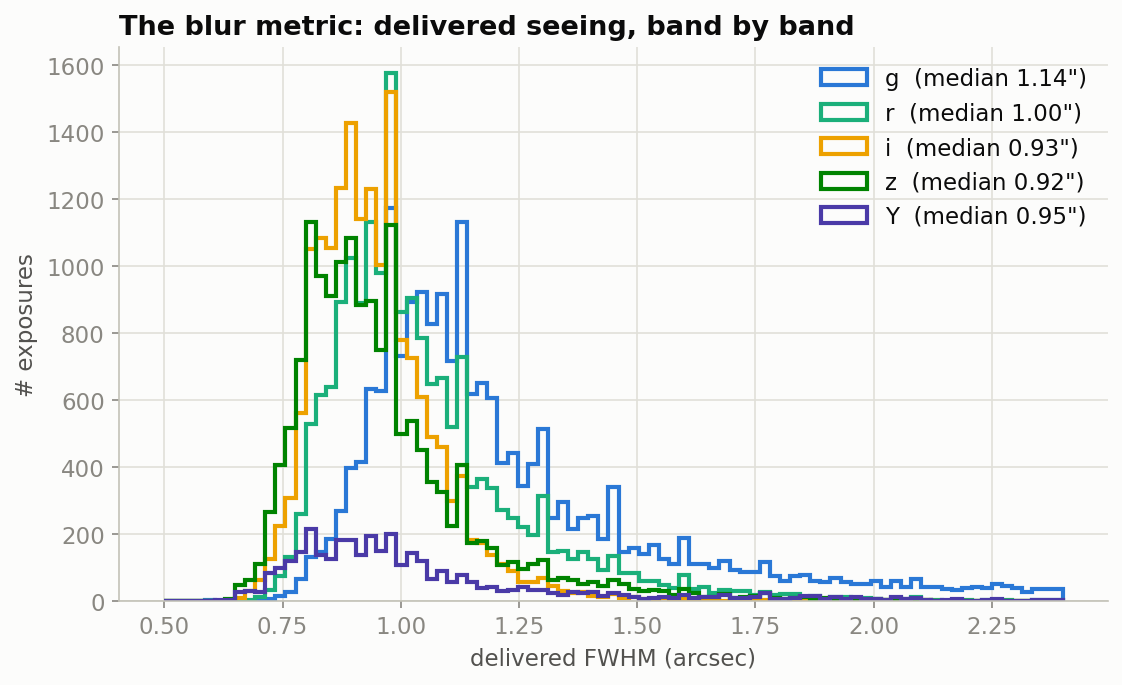
\includegraphics[width=0.85\textwidth]{blur_by_band.png}
  \caption{Delivered seeing by band: blur distributions in each DECam filter. Redder
    bands are sharper, following the $\lambda^{-0.2}$ law.}
  \label{fig:blur-by-band}
\end{figure}

\begin{figure}[htbp]
  \centering
  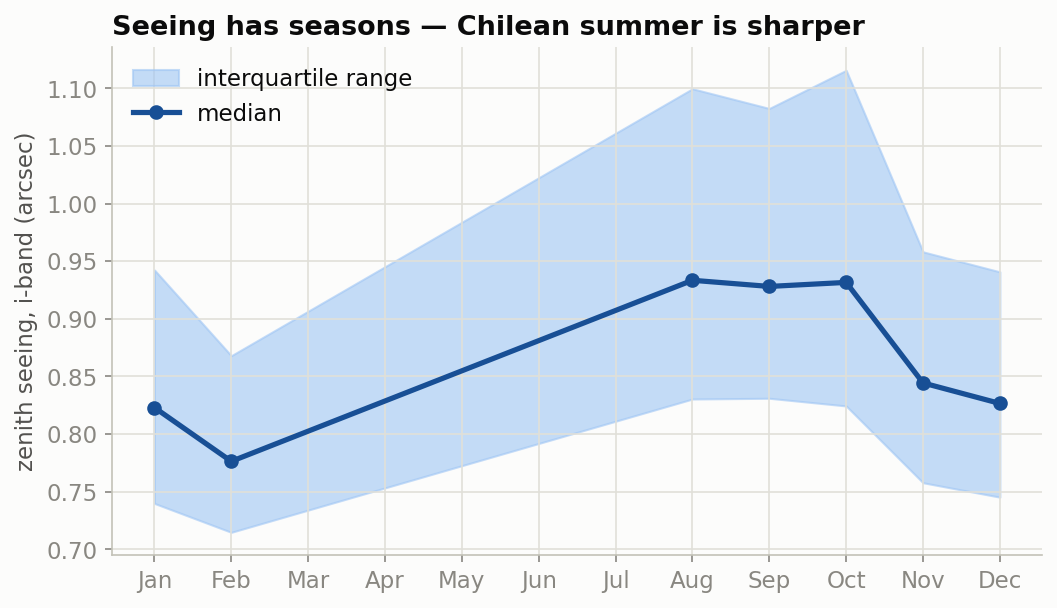
\includegraphics[width=0.85\textwidth]{seeing_seasonality.png}
  \caption{Seeing seasonality: monthly zenith seeing at CTIO. The Chilean summer
    delivers sharper images.}
  \label{fig:seeing-seasonality}
\end{figure}

\subsection{The headline finding: Simpson's paradox in the scheduler logs}
\label{sec:simpson}

Eq.~\eqref{eq:blur-decomp} makes a clean prediction: regressing $\log \fwhm$ on
$\log X$ should return a slope of $+0.6$. On the pooled DES sample it returns
\begin{equation*}
  \text{pooled fit:}\quad \fwhm \propto X^{-0.23},
\end{equation*}
i.e.\ image blur apparently \emph{improves} as the telescope points farther from
zenith. Taken at face value this contradicts atmospheric physics. The resolution is
that the data are not an experiment---they are the log of a competent scheduler
acting on the conditions. DES pointed at high airmass \emph{preferentially when the
seeing was good}: across exposures, the correlation between zenith seeing and chosen
airmass is $-0.36$. In good weather the scheduler could afford to chase fields far
from zenith (and did, to serve footprint and cadence goals); in bad weather it hugged
the zenith to salvage image quality. Conditioning away the nightly weather recovers
the physics: a within-night fixed-effects fit (each night keeps its own intercept, so
only \emph{within-night} airmass variation identifies the slope) yields an exponent
of $+0.23$, restoring the physical sign and moving substantially toward the
theoretical $+0.6$ (attenuated by intra-night seeing drifts and measurement noise).
Figure~\ref{fig:blur-airmass} shows both fits; Figure~\ref{fig:blur-decomposition}
shows the atmosphere/scheduler split and the $\teff$ fraction lost to pointing, and
Figure~\ref{fig:blur-skymap} maps delivered seeing across the DES footprint.

\begin{figure}[htbp]
  \centering
  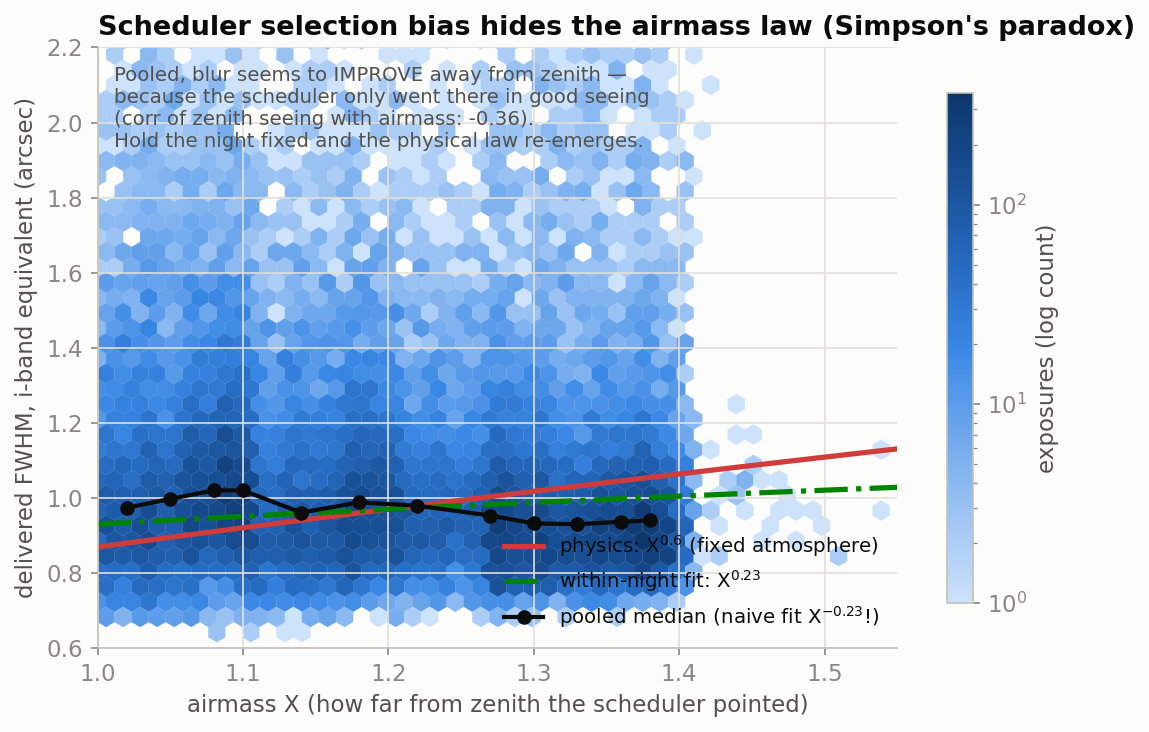
\includegraphics[width=0.9\textwidth]{blur_airmass.png}
  \caption{Scheduler selection bias as Simpson's paradox. Pooled over all exposures,
    blur seems to improve with airmass (slope $-0.23$), because the scheduler pointed
    low only in good seeing (corr(zenith seeing, airmass) $= -0.36$). Holding the
    night fixed recovers the physical $X^{0.6}$ trend (within-night slope $+0.23$).}
  \label{fig:blur-airmass}
\end{figure}

\begin{figure}[htbp]
  \centering
  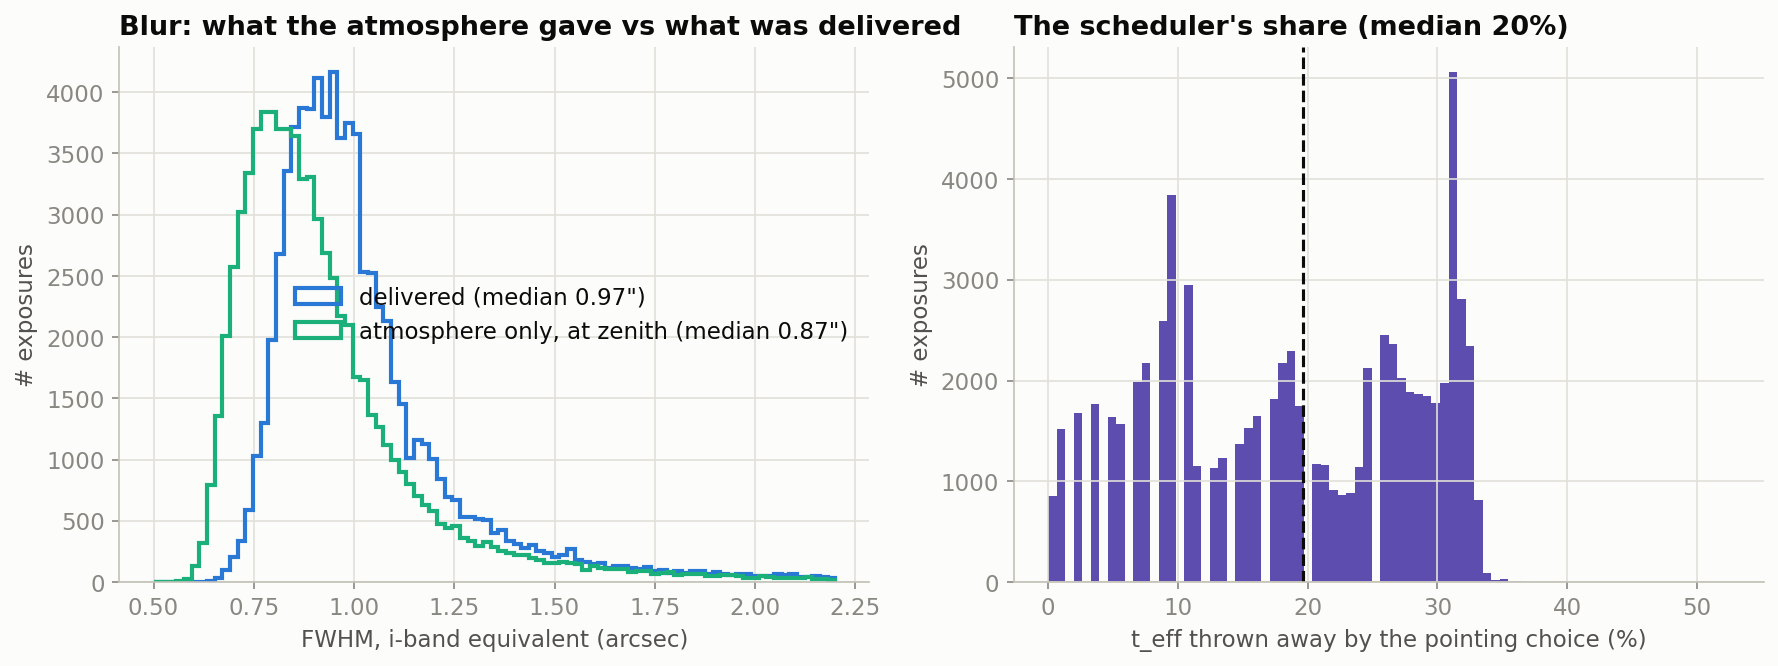
\includegraphics[width=0.9\textwidth]{blur_decomposition.png}
  \caption{Atmosphere vs.\ scheduler: zenith seeing (uncontrollable) against
    delivered blur, and the fraction of blur-term $\teff$ lost to the pointing
    decision (median 19.7\%).}
  \label{fig:blur-decomposition}
\end{figure}

\begin{figure}[htbp]
  \centering
  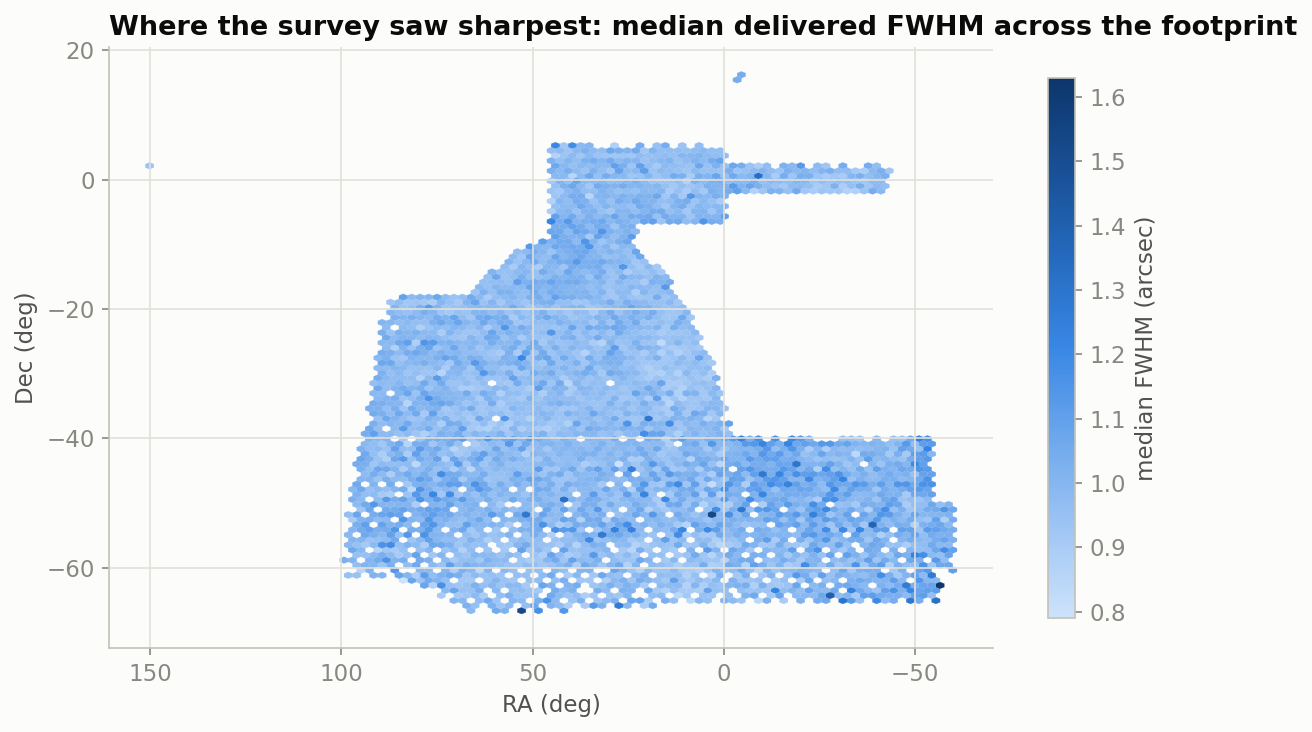
\includegraphics[width=0.75\textwidth]{blur_skymap.png}
  \caption{Median delivered FWHM across the DES footprint.}
  \label{fig:blur-skymap}
\end{figure}

This is textbook Simpson's paradox---a trend that reverses once a confounder (the
night's weather) is conditioned on---but we want to stress what it means for our
research program. The confounder here is not a nuisance of nature; \emph{it is the
logging policy itself}. Any naive evaluation of a scheduling policy against these
logs inherits the bias: a policy that points at high airmass would look spuriously
good, because in the data high-airmass exposures happen to be good-seeing exposures.
This is exactly the off-policy evaluation problem, encountered empirically in our own
data before we have trained a single agent. It sharpens the case for two design
decisions: (i) rewards and evaluation metrics must be built from the
\emph{decomposed} quantities of Eq.~\eqref{eq:blur-decomp}---credit the scheduler for
its airmass choices given the atmosphere it was dealt, never for the atmosphere
itself; and (ii) on the learning side, conservative offline-RL methods such as CQL
\citep{kumar2020}, which explicitly distrust state--action regions the logging policy
never visited, are not optional safety trimmings but responses to a bias we can now
point to in the data.

\section{From exposures to schedules: per-night metrics}
\label{sec:schedule}

\subsection{Metrics}

$\teff$ scores one exposure; a schedule is a night of sequential decisions, and its
score must also account for the time the telescope wasted \emph{between} exposures.
The bridge is Eq.~\eqref{eq:effective-seconds}: the night's effective science seconds
are $\sum \teff\,\tau$, and our headline schedule metric is the fraction of the
wall-clock night converted into fiducial-condition science time,
\begin{equation}
  \text{effective\_efficiency} \;=\; \frac{\sum_i \teff_{,i}\, \tau_i}{\text{night span}},
  \label{eq:eff-eff}
\end{equation}
where the night span runs from the first shutter-open to the last shutter-close. This
single number is degraded by \emph{either} of the two independent ways a night is
lost---sitting idle (dead time between exposures) or observing through poor
conditions---and Figure~\ref{fig:efficiency-plane} separates the two by plotting
open-shutter efficiency against mean $\teff$.

Because a single number hides \emph{why} a night scored what it did, we decompose it
into three sub-scores, each already on a $[0,1]$ scale:
\begin{itemize}
  \item \textbf{yield} --- the effective efficiency of Eq.~\eqref{eq:eff-eff}
    (capped at 1): everything combined.
  \item \textbf{quality} --- the fraction of exposures passing the DES per-band
    keep-or-retake thresholds (Table~\ref{tab:calibration};
    Figure~\ref{fig:teff-thresholds} shows the pass fractions per band across the
    survey): would this night's data actually count?
  \item \textbf{pointing} --- the mean fraction of the blur term retained given the
    airmasses the scheduler chose, $\overline{X^{-1.2}}$ (1.0 = everything at
    zenith): the sub-score that isolates the scheduler's own contribution, following
    Section~\ref{sec:blur}. Clouds and bad seeing are not its fault; airmass is a
    choice.
\end{itemize}
These combine into a composite 0--100 score as a weighted average with weights
$0.5 / 0.25 / 0.25$ (yield/quality/pointing). We state plainly: \emph{these weights
are a v0.1 proposal}, chosen to be transparent and decomposable rather than final,
and reviewing them with our mentors is the first item of Section~\ref{sec:next}. The
value of the construction is that any reweighting is a one-line change and every
score remains auditable into its three named parts.

\subsection{Results on 615 real DES nights}

Applying the metrics to the clean survey sample scores $615$ nights;
Figure~\ref{fig:night-scores} shows every night with a 60-day rolling median. The
median composite score is $64.1$, with clear seasonal structure inherited from the
seeing seasonality of Figure~\ref{fig:seeing-seasonality}.
Table~\ref{tab:nights} lists the five best and five worst nights, and
Figure~\ref{fig:best-worst} follows $\teff$ exposure-by-exposure through the extreme
nights.

\begin{table}[htbp]
  \centering
  \caption{The five best and five worst DES nights under the composite score.
    ``Eff.\ eff.''\ is the effective efficiency of Eq.~\eqref{eq:eff-eff};
    ``pass'' is the fraction of exposures meeting the DES $\teff$ thresholds;
    $X_{\mathrm{med}}$ is the median airmass.}
  \label{tab:nights}
  \begin{tabular}{lrrrrrr}
    \toprule
    Night & Score & $N_{\mathrm{exp}}$ & Mean $\teff$ & Eff.\ eff. & Pass & $X_{\mathrm{med}}$ \\
    \midrule
    \multicolumn{7}{l}{\emph{Best}} \\
    2019-01-08 & 98.3 &  34 & 1.693 & 1.190 & 1.000 & 1.06 \\
    2015-09-01 & 97.8 &  27 & 1.532 & 1.074 & 1.000 & 1.08 \\
    2018-11-26 & 96.2 & 218 & 1.659 & 1.128 & 1.000 & 1.15 \\
    2018-02-21 & 96.0 &  96 & 1.430 & 1.054 & 0.990 & 1.16 \\
    2017-12-21 & 93.8 &  63 & 1.317 & 0.992 & 1.000 & 1.28 \\
    \midrule
    \multicolumn{7}{l}{\emph{Worst}} \\
    2018-09-11 & 19.2 &  24 & 0.021 & 0.010 & 0.000 & 1.31 \\
    2016-09-14 & 20.8 &  27 & 0.068 & 0.013 & 0.000 & 1.19 \\
    2014-01-17 & 21.9 &  26 & 0.161 & 0.089 & 0.000 & 1.37 \\
    2014-10-14 & 22.9 &  77 & 0.080 & 0.041 & 0.013 & 1.19 \\
    2015-09-15 & 23.3 &  57 & 0.054 & 0.019 & 0.000 & 1.09 \\
    \bottomrule
  \end{tabular}
\end{table}

The extremes are physically sensible, which is itself a validation. The best night,
2019-01-08 (Chilean summer, near the survey's end), has a mean $\teff$ of
$1.69$---conditions \emph{better than fiducial}, so every open-shutter second was
worth 1.69 fiducial seconds, and the effective efficiency exceeds unity ($1.19$): the
night produced more fiducial-condition science time than its wall-clock span. Every
exposure passed threshold, and the median airmass of $1.06$ shows the scheduler was
also pointing well. The worst night, 2018-09-11, was simply clouded out: mean $\teff$
of $0.02$ means the shutter was open but essentially nothing came through---an
effective efficiency of $0.01$, with not one exposure passing threshold. Note that
its open-shutter efficiency ($0.50$) was unremarkable: the telescope was
\emph{operating}, just pointlessly. Only the effective efficiency, not any
shutter-time bookkeeping, captures that distinction---the efficiency plane of
Figure~\ref{fig:efficiency-plane} makes the two failure axes explicit.

\begin{figure}[htbp]
  \centering
  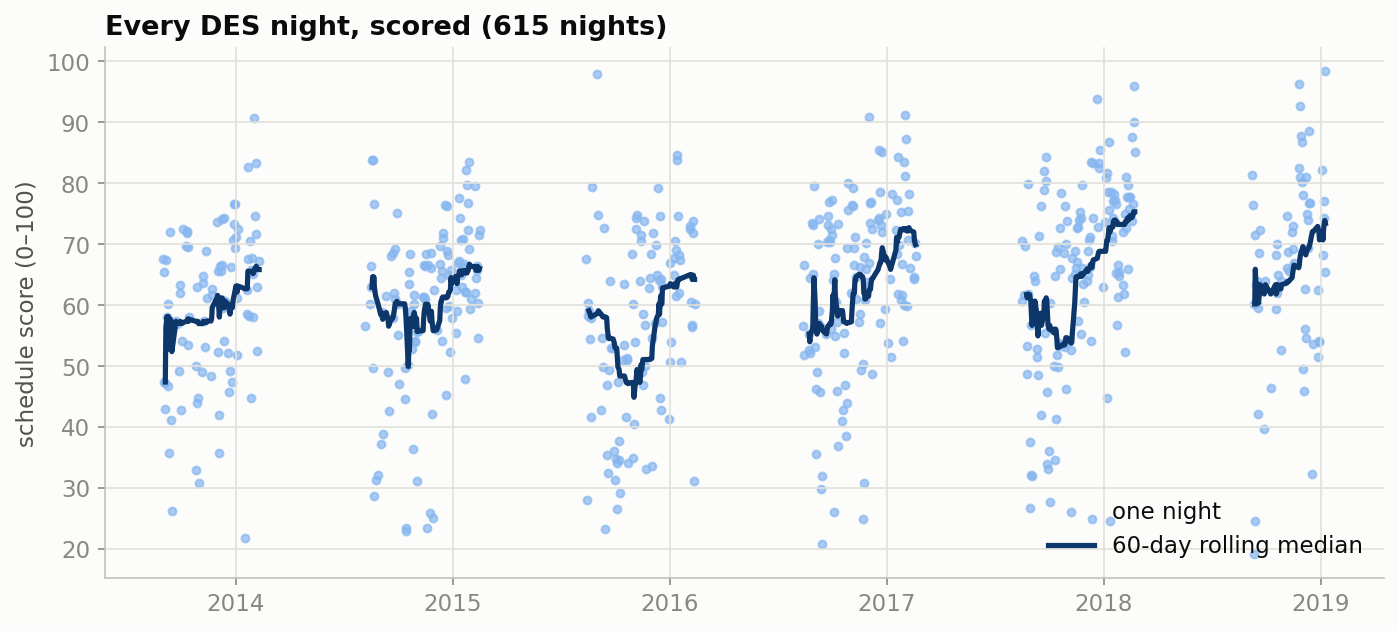
\includegraphics[width=0.95\textwidth]{night_scores.png}
  \caption{Every DES night, scored: the composite schedule score for each of the 615
    nights with a 60-day rolling median.}
  \label{fig:night-scores}
\end{figure}

\begin{figure}[htbp]
  \centering
  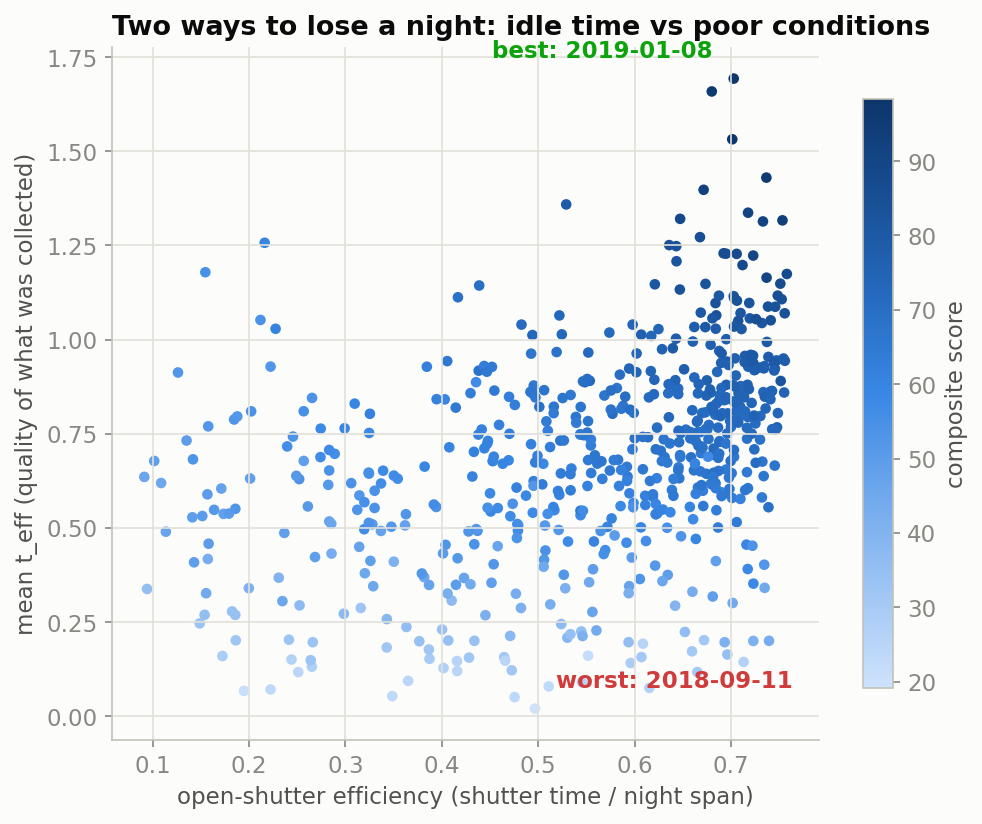
\includegraphics[width=0.8\textwidth]{efficiency_plane.png}
  \caption{The efficiency plane: idle time vs.\ poor conditions are two independent
    ways a night is lost.}
  \label{fig:efficiency-plane}
\end{figure}

\begin{figure}[htbp]
  \centering
  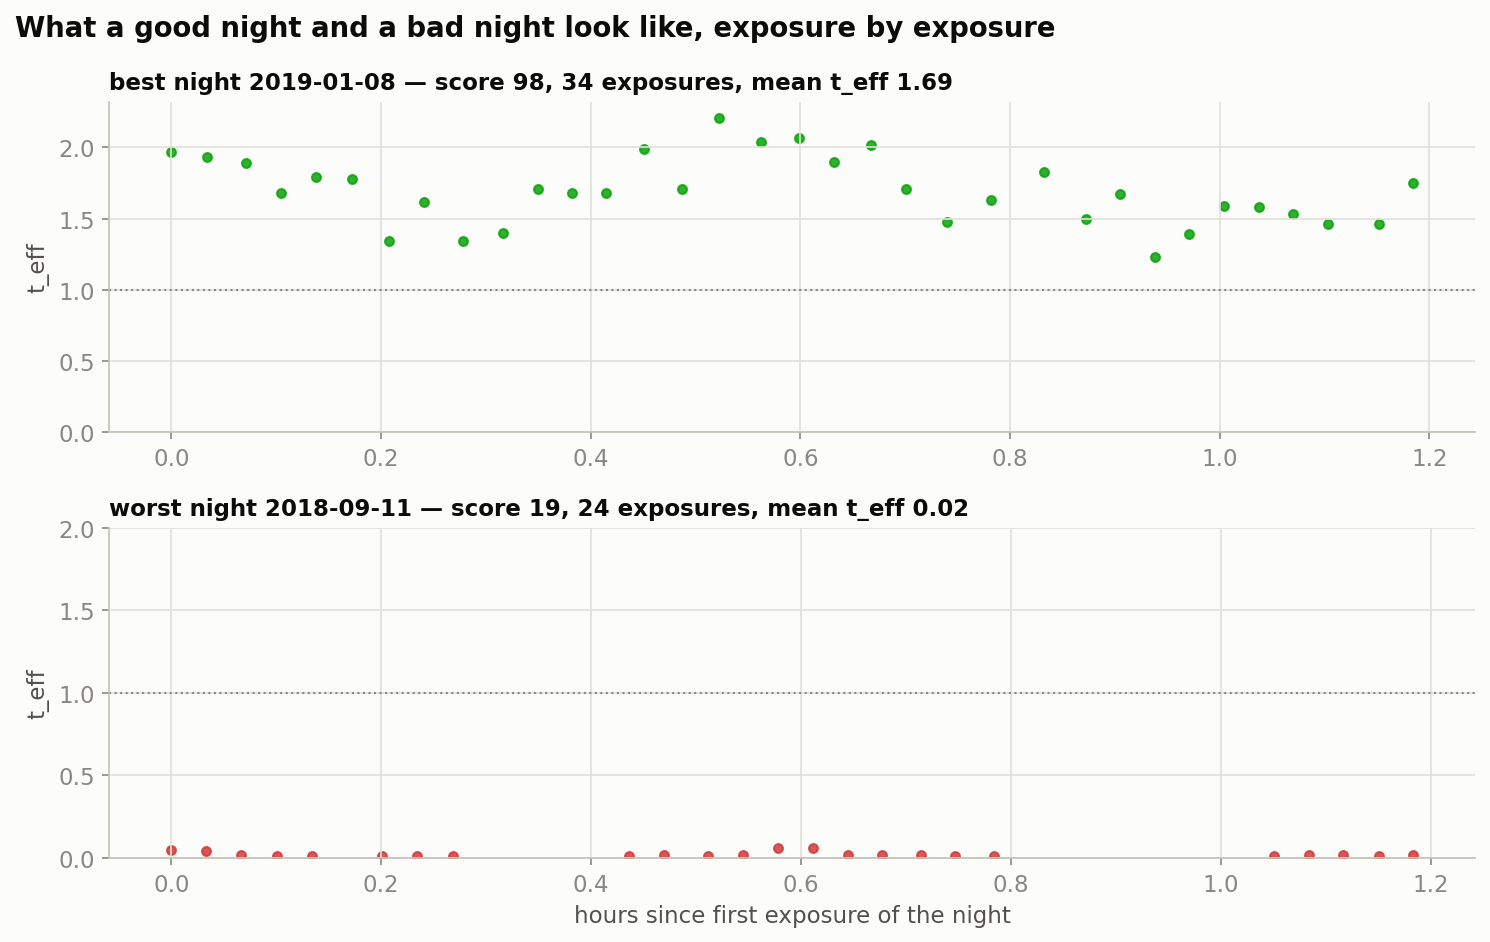
\includegraphics[width=0.95\textwidth]{best_worst_nights.png}
  \caption{Exposure-by-exposure $\teff$ through the highest- and lowest-scoring
    nights.}
  \label{fig:best-worst}
\end{figure}

\begin{figure}[htbp]
  \centering
  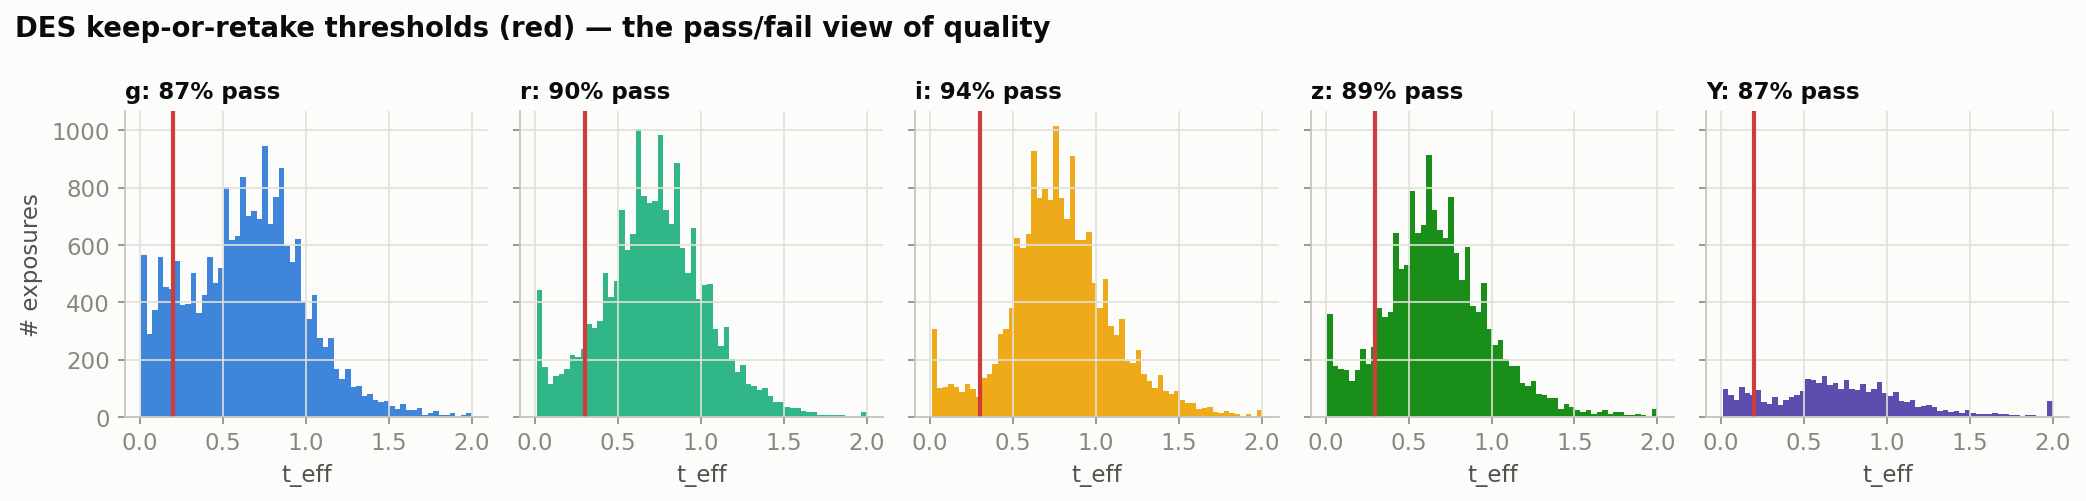
\includegraphics[width=0.85\textwidth]{teff_thresholds.png}
  \caption{Keep-or-retake: fraction of exposures meeting the DES per-band survey
    thresholds on $\teff$.}
  \label{fig:teff-thresholds}
\end{figure}

\section{Discussion and next steps}
\label{sec:next}

What this phase establishes: a per-exposure reward ($\teff$) with a first-principles
derivation, calibrated per band and validated at log-correlation $0.952$ against the
DES pipeline; a decomposition of its dominant term that separates weather from
scheduling decisions; schedule-level metrics with a transparent composite score,
exercised on 615 real nights; and a packaged, tested toolkit
(\texttt{skai\_metrics}) the group can build on. It also surfaced a finding we did
not go looking for---the airmass/seeing selection bias of
Section~\ref{sec:simpson}---which turns an abstract concern about off-policy
evaluation into a measured number in our own data.

The immediate next steps, roughly in order:

\begin{enumerate}
  \item \textbf{Review the composite weights with mentors.} The $0.5/0.25/0.25$
    split of yield/quality/pointing is a deliberate v0.1 stake in the ground. The
    sub-scores are the durable part; the weights should reflect the group's
    priorities and may end up program-dependent.
  \item \textbf{Score the group's prototype AI scheduler.} The metrics were built to
    compare schedulers, not just nights. Running the toolkit on the prototype's
    simulated output against matched DES nights is the first real test---with the
    Section~\ref{sec:simpson} caveat front and center whenever the comparison leans
    on logged conditions.
  \item \textbf{Per-program weighting.} The present scores treat all effective
    seconds equally, which is right for the wide survey but wrong across programs: a
    supernova-field visit has cadence value and a GW follow-up exposure has time
    criticality that raw $\teff\cdot\tau$ does not see. A per-program utility weight
    on Eq.~\eqref{eq:effective-seconds} is the natural extension.
  \item \textbf{Slew and dead-time modeling.} Effective efficiency penalizes dead
    time without attributing it. Modeling slew time as a function of angular
    distance between pointings would let us split dead time into ``physically
    necessary'' and ``wasted,'' giving the scheduler a sharper signal about sequence
    ordering.
  \item \textbf{Toward reward shaping for CQL.} The end state is a reward for
    conservative offline RL \citep{kumar2020}: per-step $\teff\cdot\tau$ as the
    base, with the pointing decomposition guarding against crediting weather, and
    the per-program weights encoding scientific priorities. The evaluation metrics
    of Section~\ref{sec:schedule} then serve as the held-out judge of whatever
    policy the training produces.
\end{enumerate}

The guiding principle throughout is the one that opened this note: the reward is the
foundation. We would rather spend a phase validating it against 74{,}323 real
exposures than discover, several training runs from now, that our agent has been
diligently optimizing an artifact.

\begin{thebibliography}{9}

\bibitem[Kumar et al.(2020)]{kumar2020}
Kumar, A., Zhou, A., Tucker, G., \& Levine, S.\ 2020,
``Conservative Q-Learning for Offline Reinforcement Learning,''
Advances in Neural Information Processing Systems 33,
arXiv:2006.04779.

\bibitem[Neilsen et al.(2019)]{neilsen2019}
Neilsen, E.~H., Annis, J.~T., Diehl, H.~T., et al.\ 2019,
``Dark Energy Survey's Observation Strategy, Tactics, and Exposure Scheduler,''
arXiv:1912.06254.

\bibitem[Terranova et al.(2023)]{terranova2023}
Terranova, F., Voetberg, M., Nord, B., \& \'Ciprijanovi\'c, A.\ 2023,
``Self-Driving Telescopes: Autonomous Scheduling of Astronomical Observation
Campaigns with Offline Reinforcement Learning,''
Machine Learning and the Physical Sciences Workshop, NeurIPS 2023,
arXiv:2311.18094.

\end{thebibliography}

\end{document}
